% Options for packages loaded elsewhere
\PassOptionsToPackage{unicode}{hyperref}
\PassOptionsToPackage{hyphens}{url}
\PassOptionsToPackage{dvipsnames,svgnames,x11names}{xcolor}
%
\documentclass[
  letterpaper,
  DIV=11,
  numbers=noendperiod]{scrreprt}

\usepackage{amsmath,amssymb}
\usepackage{lmodern}
\usepackage{iftex}
\ifPDFTeX
  \usepackage[T1]{fontenc}
  \usepackage[utf8]{inputenc}
  \usepackage{textcomp} % provide euro and other symbols
\else % if luatex or xetex
  \usepackage{unicode-math}
  \defaultfontfeatures{Scale=MatchLowercase}
  \defaultfontfeatures[\rmfamily]{Ligatures=TeX,Scale=1}
\fi
% Use upquote if available, for straight quotes in verbatim environments
\IfFileExists{upquote.sty}{\usepackage{upquote}}{}
\IfFileExists{microtype.sty}{% use microtype if available
  \usepackage[]{microtype}
  \UseMicrotypeSet[protrusion]{basicmath} % disable protrusion for tt fonts
}{}
\makeatletter
\@ifundefined{KOMAClassName}{% if non-KOMA class
  \IfFileExists{parskip.sty}{%
    \usepackage{parskip}
  }{% else
    \setlength{\parindent}{0pt}
    \setlength{\parskip}{6pt plus 2pt minus 1pt}}
}{% if KOMA class
  \KOMAoptions{parskip=half}}
\makeatother
\usepackage{xcolor}
\setlength{\emergencystretch}{3em} % prevent overfull lines
\setcounter{secnumdepth}{5}
% Make \paragraph and \subparagraph free-standing
\ifx\paragraph\undefined\else
  \let\oldparagraph\paragraph
  \renewcommand{\paragraph}[1]{\oldparagraph{#1}\mbox{}}
\fi
\ifx\subparagraph\undefined\else
  \let\oldsubparagraph\subparagraph
  \renewcommand{\subparagraph}[1]{\oldsubparagraph{#1}\mbox{}}
\fi


\providecommand{\tightlist}{%
  \setlength{\itemsep}{0pt}\setlength{\parskip}{0pt}}\usepackage{longtable,booktabs,array}
\usepackage{calc} % for calculating minipage widths
% Correct order of tables after \paragraph or \subparagraph
\usepackage{etoolbox}
\makeatletter
\patchcmd\longtable{\par}{\if@noskipsec\mbox{}\fi\par}{}{}
\makeatother
% Allow footnotes in longtable head/foot
\IfFileExists{footnotehyper.sty}{\usepackage{footnotehyper}}{\usepackage{footnote}}
\makesavenoteenv{longtable}
\usepackage{graphicx}
\makeatletter
\def\maxwidth{\ifdim\Gin@nat@width>\linewidth\linewidth\else\Gin@nat@width\fi}
\def\maxheight{\ifdim\Gin@nat@height>\textheight\textheight\else\Gin@nat@height\fi}
\makeatother
% Scale images if necessary, so that they will not overflow the page
% margins by default, and it is still possible to overwrite the defaults
% using explicit options in \includegraphics[width, height, ...]{}
\setkeys{Gin}{width=\maxwidth,height=\maxheight,keepaspectratio}
% Set default figure placement to htbp
\makeatletter
\def\fps@figure{htbp}
\makeatother
\newlength{\cslhangindent}
\setlength{\cslhangindent}{1.5em}
\newlength{\csllabelwidth}
\setlength{\csllabelwidth}{3em}
\newlength{\cslentryspacingunit} % times entry-spacing
\setlength{\cslentryspacingunit}{\parskip}
\newenvironment{CSLReferences}[2] % #1 hanging-ident, #2 entry spacing
 {% don't indent paragraphs
  \setlength{\parindent}{0pt}
  % turn on hanging indent if param 1 is 1
  \ifodd #1
  \let\oldpar\par
  \def\par{\hangindent=\cslhangindent\oldpar}
  \fi
  % set entry spacing
  \setlength{\parskip}{#2\cslentryspacingunit}
 }%
 {}
\usepackage{calc}
\newcommand{\CSLBlock}[1]{#1\hfill\break}
\newcommand{\CSLLeftMargin}[1]{\parbox[t]{\csllabelwidth}{#1}}
\newcommand{\CSLRightInline}[1]{\parbox[t]{\linewidth - \csllabelwidth}{#1}\break}
\newcommand{\CSLIndent}[1]{\hspace{\cslhangindent}#1}

\usepackage{amsmath}
\usepackage{booktabs}
\usepackage{caption}
\usepackage{longtable}
\KOMAoption{captions}{tableheading}
\makeatletter
\@ifpackageloaded{tcolorbox}{}{\usepackage[many]{tcolorbox}}
\@ifpackageloaded{fontawesome5}{}{\usepackage{fontawesome5}}
\definecolor{quarto-callout-color}{HTML}{909090}
\definecolor{quarto-callout-note-color}{HTML}{0758E5}
\definecolor{quarto-callout-important-color}{HTML}{CC1914}
\definecolor{quarto-callout-warning-color}{HTML}{EB9113}
\definecolor{quarto-callout-tip-color}{HTML}{00A047}
\definecolor{quarto-callout-caution-color}{HTML}{FC5300}
\definecolor{quarto-callout-color-frame}{HTML}{acacac}
\definecolor{quarto-callout-note-color-frame}{HTML}{4582ec}
\definecolor{quarto-callout-important-color-frame}{HTML}{d9534f}
\definecolor{quarto-callout-warning-color-frame}{HTML}{f0ad4e}
\definecolor{quarto-callout-tip-color-frame}{HTML}{02b875}
\definecolor{quarto-callout-caution-color-frame}{HTML}{fd7e14}
\makeatother
\makeatletter
\makeatother
\makeatletter
\@ifpackageloaded{bookmark}{}{\usepackage{bookmark}}
\makeatother
\makeatletter
\@ifpackageloaded{caption}{}{\usepackage{caption}}
\AtBeginDocument{%
\ifdefined\contentsname
  \renewcommand*\contentsname{Tabla de contenidos}
\else
  \newcommand\contentsname{Tabla de contenidos}
\fi
\ifdefined\listfigurename
  \renewcommand*\listfigurename{Listado de Figuras}
\else
  \newcommand\listfigurename{Listado de Figuras}
\fi
\ifdefined\listtablename
  \renewcommand*\listtablename{Listado de Tablas}
\else
  \newcommand\listtablename{Listado de Tablas}
\fi
\ifdefined\figurename
  \renewcommand*\figurename{Figura}
\else
  \newcommand\figurename{Figura}
\fi
\ifdefined\tablename
  \renewcommand*\tablename{Tabla}
\else
  \newcommand\tablename{Tabla}
\fi
}
\@ifpackageloaded{float}{}{\usepackage{float}}
\floatstyle{ruled}
\@ifundefined{c@chapter}{\newfloat{codelisting}{h}{lop}}{\newfloat{codelisting}{h}{lop}[chapter]}
\floatname{codelisting}{Listado}
\newcommand*\listoflistings{\listof{codelisting}{Listado de Listados}}
\makeatother
\makeatletter
\@ifpackageloaded{caption}{}{\usepackage{caption}}
\@ifpackageloaded{subcaption}{}{\usepackage{subcaption}}
\makeatother
\makeatletter
\@ifpackageloaded{tcolorbox}{}{\usepackage[many]{tcolorbox}}
\makeatother
\makeatletter
\@ifundefined{shadecolor}{\definecolor{shadecolor}{rgb}{.97, .97, .97}}
\makeatother
\makeatletter
\makeatother
\ifLuaTeX
\usepackage[bidi=basic]{babel}
\else
\usepackage[bidi=default]{babel}
\fi
\babelprovide[main,import]{spanish}
% get rid of language-specific shorthands (see #6817):
\let\LanguageShortHands\languageshorthands
\def\languageshorthands#1{}
\ifLuaTeX
  \usepackage{selnolig}  % disable illegal ligatures
\fi
\IfFileExists{bookmark.sty}{\usepackage{bookmark}}{\usepackage{hyperref}}
\IfFileExists{xurl.sty}{\usepackage{xurl}}{} % add URL line breaks if available
\urlstyle{same} % disable monospaced font for URLs
\hypersetup{
  pdftitle={Informe Encuesta Metodología y Técnicas Cuantitativas},
  pdfauthor={Metodología Cuantitativa},
  pdflang={es},
  colorlinks=true,
  linkcolor={blue},
  filecolor={Maroon},
  citecolor={Blue},
  urlcolor={Blue},
  pdfcreator={LaTeX via pandoc}}

\title{Informe Encuesta Metodología y Técnicas Cuantitativas}
\author{Metodología Cuantitativa}
\date{15/2/23}

\begin{document}
\maketitle
\ifdefined\Shaded\renewenvironment{Shaded}{\begin{tcolorbox}[enhanced, breakable, borderline west={3pt}{0pt}{shadecolor}, frame hidden, interior hidden, sharp corners, boxrule=0pt]}{\end{tcolorbox}}\fi

\renewcommand*\contentsname{Tabla de contenidos}
{
\hypersetup{linkcolor=}
\setcounter{tocdepth}{2}
\tableofcontents
}
\bookmarksetup{startatroot}

\hypertarget{presentaciuxf3n-y-objetivos-del-informe}{%
\chapter*{Presentación y objetivos del
informe}\label{presentaciuxf3n-y-objetivos-del-informe}}
\addcontentsline{toc}{chapter}{Presentación y objetivos del informe}

\markboth{Presentación y objetivos del informe}{Presentación y objetivos
del informe}

El siguiente informe tiene una finalidad principalmente pedagógica.
Específicamente está pensado como un mecanismo para ayudar a alcanzar
los siguientes objetivos que forman parte del
\href{https://docs.google.com/document/d/15ZuHJ1ZM7Z0g0Edt-mv1PCB697-x6-rZfcWdAtd85yM/edit\#heading=h.s43n504lcmmx}{programa}
de la materia ``Metodología y Técnicas Cuantitativas'' de la UNAJ:

\begin{itemize}
\item
  Lograr un conocimiento mínimo de la existencia y pertinencia de las
  técnicas de análisis de datos \emph{básicas} y una \emph{habilidad}
  mínima en la ejecución de las mismas.
\item
  \emph{Lograr un} conocimiento mínimo de la existencia y pertinencia de
  (otras) técnicas de análisis de datos más específicas y (usualmente)
  más \emph{complejas}.
\end{itemize}

Aparte de la distinción entre técnicas básicas y complejas la diferencia
en cuanto a los objetivos pedagógicos es que entre ambos objetivos es
que las últimas sólo se aspira a conocerlas mientras que en las primeras
se espera, también, que se adquiera cierta habilidad en su ejecución.
Expresado de otro modo, de las técnicas consideradas complejas se espera
que se sepa de su existencia y qué tipos de problemas ayuda a
solucionar. En cambio, en las técnicas básicas se espera lo anterior
pero que además se adquiera la habilidad de poder ejecutar las mismas.

Para lograr lo anterior durante la cursada de la materia se realiza una
encuesta mediante un
\href{https://www.google.com/intl/es-419_ar/forms/about/}{formulario de
google} que contestan los mismos estudiantes. Luego el contenido de sus
respuestas se analiza con el \href{https://www.r-project.org/}{lenguaje
R} y con el mismo se escribe y publica este informe.

En cuanto al estilo del texto será deliberamente informal aunque con 3
excepciones con fines principalmente pedagógicos:

\begin{itemize}
\item
  Se incluirán piezas de código
\item
  Se hará uso de citas y referencias (estilo APA)
\item
  Los conceptos importantes apareceran traducidos al ingles entre
  paréntesis.
\end{itemize}

Por otro lado, el texto estará acompañado de los siguientes elementos
visuales:

\bookmarksetup{startatroot}

\hypertarget{diseuxf1o-de-la-encuesta}{%
\chapter{Diseño de la encuesta}\label{diseuxf1o-de-la-encuesta}}

En el diseño de la encuesta que contestan los estudiantes se pueden
distinguir 2 grandes procesos. Uno referido al diseño del cuestionario y
otro referido al diseño de la selección de los casos. El primero se
preocupa por \textbf{qué se pregunta} y el segundo por \textbf{a
quienes}. En esta sección la mayoría de las veces sólo se explicitará
pero pocas veces se justificará las decisiones tomadas en ambos
procesos. En otras palabras, la palabra ``diseño'' le queda grande a
ambos procesos para esta encuesta. Lamentablemente lo mismo puede
afirmarse de varias encuestas académicas o profesionales. La
justificación particular para la falta de atención metodológica a estos
puntos es que en este caso se trata de una actividad con fines
principalmente pedagógicos más que académicos o profesionales.

\hypertarget{diseuxf1o-del-cuestionario}{%
\section{Diseño del cuestionario}\label{diseuxf1o-del-cuestionario}}

El
\href{https://drive.google.com/file/d/1nbU16-b2RxvPQZV2SS-Aodl1d7zPr9Cw/view?usp=sharing}{cuestionario},
como muchos cuestionarios que se usan en la práctica profesional, está
diseñado con la lógica de módulos. Como veremos más adelante en esta
instancia cada módulo tiene una justificable lógica interna pero lo que
no tiene este cuestionario es una coherencia interna que explique la
relación entre los diferentes módulos.

El diseño de un cuestionario mediante la estrategia de módulos suele ser
útil tanto para el encuestado como para el investigador. Al encuestado
lo ayuda a ordenarse visualmente especialmente si se trata de un
cuestionario largo. Al investigador lo ayuda tanto para el
etiquetamiento (o nombramiento) como para el orden de las variables en
la base de datos.

El cuestionario por ahora cuenta con los siguientes módulos:

\begin{enumerate}
\def\labelenumi{\arabic{enumi}.}
\item
  Identificación
\item
  Demográfico
\item
  Composición del hogar
\item
  Cuidados
\item
  Vivienda
\item
  Uso del tiempo
\item
  Inseguridad alimentaria
\item
  Preferencias sociales
\item
  Origen social
\item
  Trabajo actual
\item
  Ingresos del hogar
\item
  Académico UNAJ
\item
  Expectativas materia cuantitativa
\item
  Redes sociales entre estudiantes de la materia
\end{enumerate}

Claramente no parece haber mucha relación entre los diferentes módulos.
A diferencia de algunas encuestas ómnibus en donde este problema se
presenta porque cada investigador que forma parte de la investigación
agrega su propio ``paquete de preguntas'' para su particular
investigación en este caso la justificación es que cada módulo tiene una
función pedagógica particular.\footnote{En una investigación ómnibus
  varios investigadores (o clientes) comparten el mismo diseño de
  selección de casos y de esa manera, juntos, pueden llegar a más casos
  ya que entre todos amortizan estos costos que suelen ser grandes en
  encuestas grandes presenciales. A cambio, más allá de un algunos
  módulos comunes (p.e. el demográfico), cada investigador o cliente
  agrega su módulo de particular interés.}

\hypertarget{diseuxf1o-de-la-selecciuxf3n-de-casos}{%
\section{Diseño de la selección de
casos}\label{diseuxf1o-de-la-selecciuxf3n-de-casos}}

En cuanto al criterio utilizado para la selección de los casos se puede
afirmar que se trata de una muestra de los estudiantes de la materia
``Metodología y Técnicas Cuantitativas'' de la carrera de Trabajo Social
de la Universidad Nacional Arturo Jauretche. Esto ya afirma algo pero se
puede especificar aún más.

Antes que nada, si bien es una encuesta que potencialmente les llega a
todos los estudiantes que cursan la materia, la misma efectivamente sólo
llega a una muestra de los mismos. Esto se produce principalmente por la
no-respuesta de algunos estudiantes que comienzan la cursada pero no
responden la encuesta. El factor ``deserción'' no parece afectar tanto a
la selección de casos dado que la encuesta se realiza al principio de la
cursada. Esto hace que la encuesta, si es representativa de algo, lo sea
de la población intermedia que queda conformada entre los inscriptos a
la materia y los que finalmente la regularizan. Obviamente esto no
alcanza para decir mucho acerca de la representatividad de la encuesta
sobre poblaciones mayores compuestas por:

\begin{itemize}
\item
  Los estudiantes de la carrera de Trabajo Social de la UNAJ.
\item
  Los estudiantes de la UNAJ
\item
  Los estudiantes del sistema universitario nacional
\end{itemize}

\bookmarksetup{startatroot}

\hypertarget{cross}{%
\chapter{Limpieza y consistencia de los datos}\label{cross}}

El producto de los procesos de producción y registro de los datos suele
cristalizarce en una (o varias) bases de datos. Estas pueden (y suelen)
contener diferentes tipos de errores por lo que se considera una buena
práctica realizar un proceso de limpieza y preparación para recién
después comenzar el proceso estricto del análisis de los mismas.

En esta sección veremos algunos ejemplos tanto de limpieza, consistencia
y construcción de nuevas variables. Aquí veremos ejemplos de los casos
mas sencillos. Procesos como el pegado (\emph{joint}) de variables,
necesario cuando los datos se encuentran en diferentes archivos o bases
de datos, no se verán aquí.

\hypertarget{limpieza}{%
\section{Limpieza}\label{limpieza}}

La idea de limpieza (\emph{cleaning}) viene de usar la metáfora de dato
sucio (\emph{dirty}). Un dato sucio no necesariamente es un dato
incorrecto aunque sí se trata de un tipo de dato más incómodo de
trabajar ya que dificulta el posterior análisis.

La tarea de la limpieza de una base de datos suele implicar un tiempo,
especialmente en bases de datos con muchas variables (muchas columnas).
Si bien es una práctica recomendada siempre hay que tener en cuenta la
``escala'' del trabajo a realizar porque que en algunas situaciones
puede que sea más simple corregir algunas cuestiones de manera artesanal
o a mano en el proceso mismo de la publicación de los análisis. Esto
suele ser particularmente cierto en algunos de los siguientes escenarios
y sus posibles combinaciones:

\begin{itemize}
\item
  Encuestas con muchas preguntas en donde se sabe que se van a analizar
  una sola vez o que se analiza sólo una pequeña parte de la información
  disponible.
\item
  Base de datos y procesos de análisis que luego no se van a compartir
  (los resultados se comparten pero estos no son replicables por
  terceros)
\end{itemize}

De manera complementaria el proceso de limpieza se amortiza
considerablemente cuando los datos se van a analizar más de una vez y
cuando se requiere un grado de transparencia que exige que la
investigación sea enteramente replicable.

\hypertarget{renombre-de-las-variables}{%
\subsection{Renombre de las variables}\label{renombre-de-las-variables}}

La tarea básica de limpieza (\emph{cleaning}) que aquí se hará será el
\textbf{remombre de todas las variables}. La razón de esta operación es
que, al menos si se trabaja con google forms (aunque algo similar suele
suceder con otros sistemas de formularios online), los nombres de las
variables son el texto de la propia pregunta del formulario. Esto
incomoda un poco el análisis de los datos por la gran extensión de
algunas preguntas y esa incomodidad se traduce en una mayor propensión
al error. En este sentido para trabajar con los nombres de las variables
suele ser recomendable:

\begin{itemize}
\item
  Eliminar los espacios entre las palabras agregando algún símbolo que
  las pegue o una (``\_'', ``-'' o cualquier otro),
\item
  Pasar todas las letras a minúscula (o mayúscula)
\item
  Renombrar el nombre original con un nombre más corto y recordable. Una
  opción recomendable es que cuando en la encuesta haya variables que
  corresponde a un mismo módulo (p.e. módulo vivienda) se inicien por un
  mismo prefijo (viv\_habitaciones, viv\_inodoro, etc.).
\end{itemize}

\hypertarget{orden-de-las-variables}{%
\subsection{Orden de las variables}\label{orden-de-las-variables}}

Otra tarea diferente pero relacionada con la anterior tiene que ver con
el \textbf{orden de las variables} en la base de datos. En algunos
sistemas el orden de las variables tiene que ver con el orden
cronológico en que se fueron construyendo las preguntas (p.e. en una
encuesta) o con el orden en que luego se fueron construyendo variables
complejas o recategoriaciones. En cualquier caso, lo que se debe tratar
de lograr es que las variables que tienen relación temática entre sí, no
sólo tengan un prefijo que las una sino que se encuentren visualmente
cercanas en la base de datos. Esta recomendación es más importante
cuanto más variables tenga la base de datos.

\hypertarget{etiquetado-de-las-variables}{%
\subsection{Etiquetado de las
variables}\label{etiquetado-de-las-variables}}

Antes se habló de renombrar y ordenar las variables. Sin embargo, en las
ciencias sociales y en especial en aquellas disciplinas donde se
encuentren difundidos programas estadísticos como el SPSS, SAS y Stata
se usa la distinción entre \textbf{nombre de la variable y etiqueta de
la misma}. El primero es como el nombre real de la variable y así lo
entiende el mismo programa. La segunda es como un alias o un metadato
que permite una interpretación más humana del significado de la
variable. Muchas veces el contenido de la etiqueta se acerca a la
pregunta original. Ahora bien, las variables, especialmente las que se
suelen denomianar discretas o categóricas, aparte de tener un nombre
pueden contener una serie finita de categorías.

Cuando se trata de variables del tipo ``Indique su cantidad de hijes''
si la respuesta de la base de datos es un ``2'' se entiende que la
persona ha respondido que tiene 2 hijes. Lo mismo si aparece un ``1'' o
un ``3''. Se dice que estos son los \textbf{valores} de las variables.
Pero el problema comienza, siguiendo una vieja tradición del análisis de
datos (ver ``De donde vienen las etiquetas'') cuando como respuesta a
variables del tipo ``Indique su género'' nos encontramos con símbolos
(más precisamente numerales) como ``1'', ``2'', etc. en la base de
datos. Estos símbolos se suelen llamar \textbf{códigos} y, sin
información externa, no hay manera de saber que significan. Para eso
vuelven en nuestra ayuda las etiquetas

Así como hay etiquetas para los nombres de las variables también lo hay
para sus etiquetas.

La etiqueta es especialmente útil en los contextos de presentación de
los análisis sea tanto en formato de tablas y gráficos. La razón es que
el lector de los informes puede no estar al tanto ni del cuestionario
original ni de la propia base de datos. Simplemente es un lector de un
informe que desea, razonablemente, que en vez de algo como ``n\_hijes''
apareza algo como ``Cantidad de hijes'' o que en vez de ``3'' en los
análisis de la variable ``Género'' aparezca algo como ``género no
binario''.

\hypertarget{tipo-de-dato-de-la-variable}{%
\subsection{Tipo de dato de la
variable}\label{tipo-de-dato-de-la-variable}}

Otro punto a destacar es lo que a veces de suele denominar ``nivel de
medición'' de la variable. Este término se suele utilizar más en
programas o lenguajes específicos para análisis de datos pero tienen una
similitud con el proceso usual en una planilla de cálculo (excel, google
sheet, etc) de aplicarle ``formato'' a la celda para indicarle si se
trata de texto o un número y sí se trata de número de que tipo
(porcentaje, fecha, decimal, etc.).

Este tipo de metainformación suele ser útil para que el programa detecte
que tipo de gráfico es apropiado o que tipo de cálculo realizar. De
todos modos los programas vienen cada vez con mejores heurísticas para
adiviniar, sin previa indicación de que tipo de dato se trata.

\bookmarksetup{startatroot}

\hypertarget{anuxe1lisis-espaciales}{%
\chapter{Análisis Espaciales}\label{anuxe1lisis-espaciales}}

La cartografía, la disciplina que se encarga de la confección y uso de
mapas, es una actividad milenaria. Sin embargo, desde hace relativamente
pocas décadas se ha comenzado a difundir el uso de técnicas que, no sólo
representan a diferentes objetos en un mapa, sino que tambien, al mismo
tiempo, permiten la realización de diferentes análisis específicamente
espaciales.

Los mapas pueden considerarse como una representación gráfica basada en
una proyección, que ``proyecta'' sobre un plano de 2 dimensiones (2D)
una realidad tridimensional (3D). Esta representación permite hacer
visible relaciones de distancia entre elementos en algún espacio. En
particular, los mapas geográficos (o cartográficos) suponen unas
propiedades métricas que dependen de la proyección utilizada, y
posibilitan la toma de medidas de distancias, ángulos o superficies
sobre él y su posterior (re)proyección a la realidad.

En la antigüedad, cuando sólo se sabía la ubicación específica de pocos
elementos (no había GPS), se confiaba en la representación gráfica
realizada sobre un plano (mapa) construido sobre esas (pocas)
ubicaciones conocidas y se calculaba la posición de los elementos
todavía no posicionados, sea tanto una nueva ciudad conocida o la propia
ubicación de un viajante.

\begin{tcolorbox}[enhanced jigsaw, colback=white, title=\textcolor{quarto-callout-note-color}{\faInfo}\hspace{0.5em}{Los mapas en la historia}, breakable, colbacktitle=quarto-callout-note-color!10!white, opacityback=0, opacitybacktitle=0.6, titlerule=0mm, toprule=.15mm, toptitle=1mm, leftrule=.75mm, rightrule=.15mm, bottomrule=.15mm, arc=.35mm, coltitle=black, bottomtitle=1mm, left=2mm, colframe=quarto-callout-note-color-frame]

En la actualidad, gracias a la tecnología satelital, se puede tener
información de la ubicación específica de (casi) todo lo que a uno le
interese y . De todos modos, la parte conceptual que se encuentra por
detrás de lo anterior es sumamente antigua y En efecto, su creador fue
nuestro viejo amigo
\href{https://diegoteca.com.ar/metodocuanti/?p=188}{Eratóstenes}. Él
ideó lo que se considera el primer sistema de coordenadas geográfica en
donde, bajo el supuesto de la esferidad perfecta (un cuerpo), con sólo 2
datos se podría determinar cualquier posición.

\begin{figure}[H]

{\centering 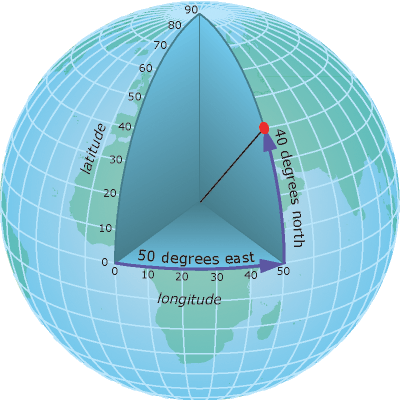
\includegraphics{./Inputs/Images/coordenadas.gif}

}

\caption{Sistemas de coordenadas teniendo como referencia una esfera o
algún tipo de elipsoide.}

\end{figure}

De modo conceptualmente independiente, para localizar esa posición en un
mapa de 2 dimensiones (plano) se requiere una proyección, esto es,~una
relación ordenada entre los puntos de la superficie curva de la~Tierra,
(o en general de cualquier cuerpo) y los de un mapa, (o en general de
cualquier plano).

\begin{figure}[H]

{\centering 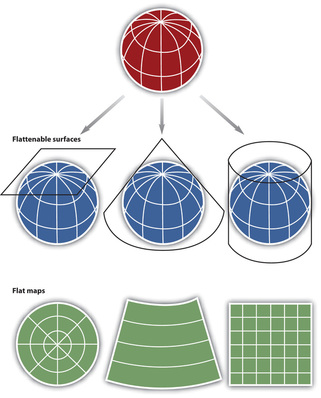
\includegraphics{./Inputs/Images/map-projections.jpg}

}

\caption{Proyecciones genéricas. La 3ra es la más similar a la usual
proyección de Mercator}

\end{figure}

Es este sentido, es importante aclarar que todo mapa geográfico de 2
dimensiones implica alguna proyección y que, dependiendo cual sea está
última, genera un tipo de distorsión específica. La distorsión se genera
al pasar de un mundo con 3 dimensiones (cuerpo geométrico) a un plano
con 2 dimensiones (figura geométrica). Por ejemplo la
\href{https://es.wikipedia.org/wiki/Proyecci\%C3\%B3n_de_Mercator}{proyección
Mercator}, la usual cuando un@ va (¿o iba?) a una librería a comprar un
mapa n° 3, supone que Groenlandia aparece aproximadamente del tamaño de
África, cuando en realidad el área de África es aproximadamente 14 veces
la de Groenlandia. Lo anterior no sucede en los globos terráqueos ya que
estos no son proyecciones.

\begin{figure}[H]

{\centering 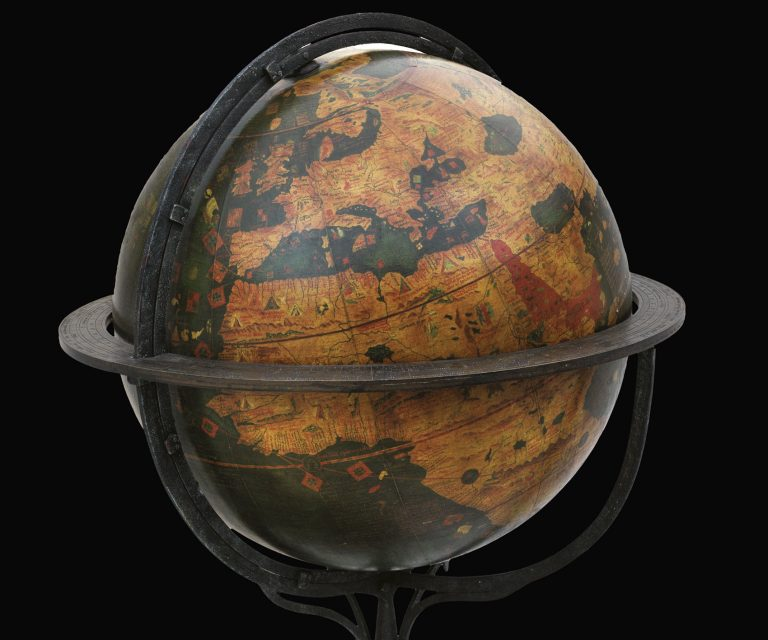
\includegraphics{./Inputs/Images/erdapfel-1492-768x640.jpg}

}

\caption{El erdapfel es el globo terráqueo más antiguo que aún se
conserva. Lo construyó un cartógrafo alemán llamado Martin Behaim en
1492}

\end{figure}

Aún con sus imperfecciones , los mapas planos también son de gran
utilidad por fuera de la navegación. En efecto, pueden servir para hacer
observables hechos que antes no lo eran, así como para el diseño,
ejecución y evaluación de políticas territoriales. Por ejemplo,
\href{https://es.wikipedia.org/wiki/John_Snow}{John Snow}, uno de los
fundadores de la epidemiología, logró trazar el origen del cólera
siguiendo la pista de los enfermos a través de un mapa. Con esta ayuda
hipotetizó que el agua en mal estado era un vector importante en la
propagación de la enfermedad cuando por aquel entonces se suponía que el
cólera (al igual que la peste bubónica) tenía que ver con la polución
del aire más que con el agua.

Snow llegó a su conclusión luego de «georeferenciar» los fallecimientos
(gracias a que un cura amigo averiguó donde vivía esa gente!) y observar
la cercanía de la mayor cantidad de muertes con una bomba manual de agua
pública. Recomendó retirar la manija de la bomba y a los pocos días la
epidemia cesó. Posteriormente se supo que los desechos de uno de los
pozos ciegos de las casas linderas se había filtrado hacia la capa
freática que la bomba extraía el agua.

\begin{figure}[H]

{\centering 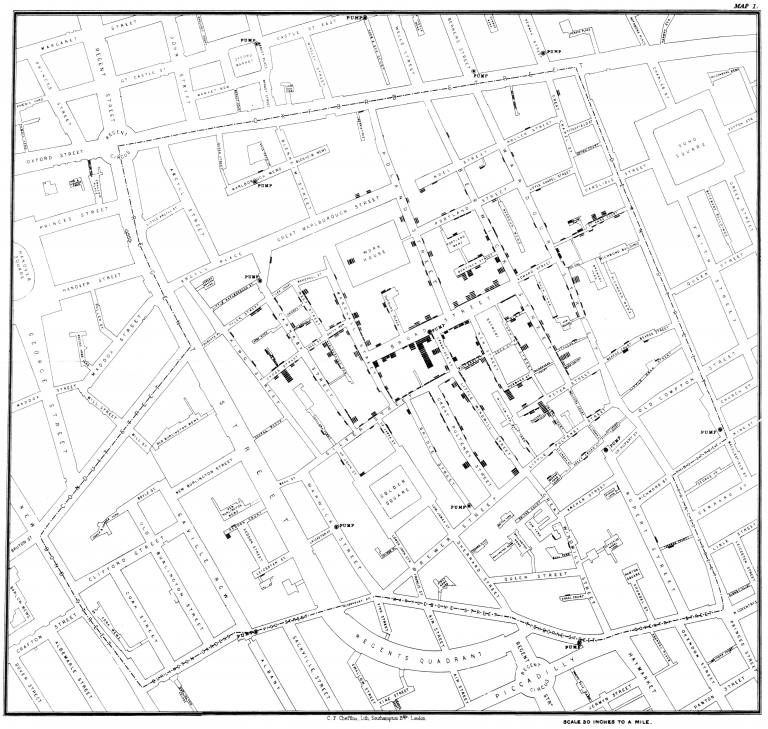
\includegraphics{./Inputs/Images/snowmap-1854-768x729.png}

}

\caption{Mapa original de John Snow (1854). Los puntos negros simbolizan
fallecimientos.}

\end{figure}

\end{tcolorbox}

\hypertarget{insumos-de-la-encuesta}{%
\section{Insumos de la encuesta}\label{insumos-de-la-encuesta}}

Los principales análisis que se muestran a continuación se basan en una
serie de preguntas del módulo de vivienda que refieren a la dirección de
la misma como la calle, la altura y el partido o departamento del
estudiante.

\begin{figure}

{\centering 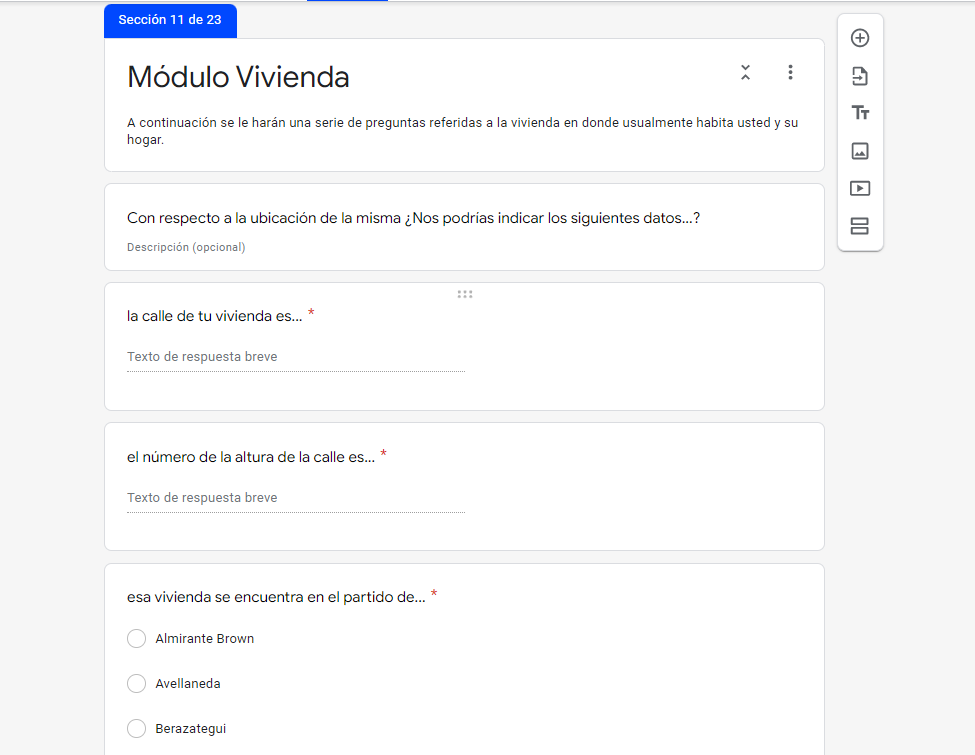
\includegraphics[width=6.25in,height=\textheight]{./Inputs/Images/pregunta_geo.png}

}

\caption{pregunta\_ubicacion\_vivienda}

\end{figure}

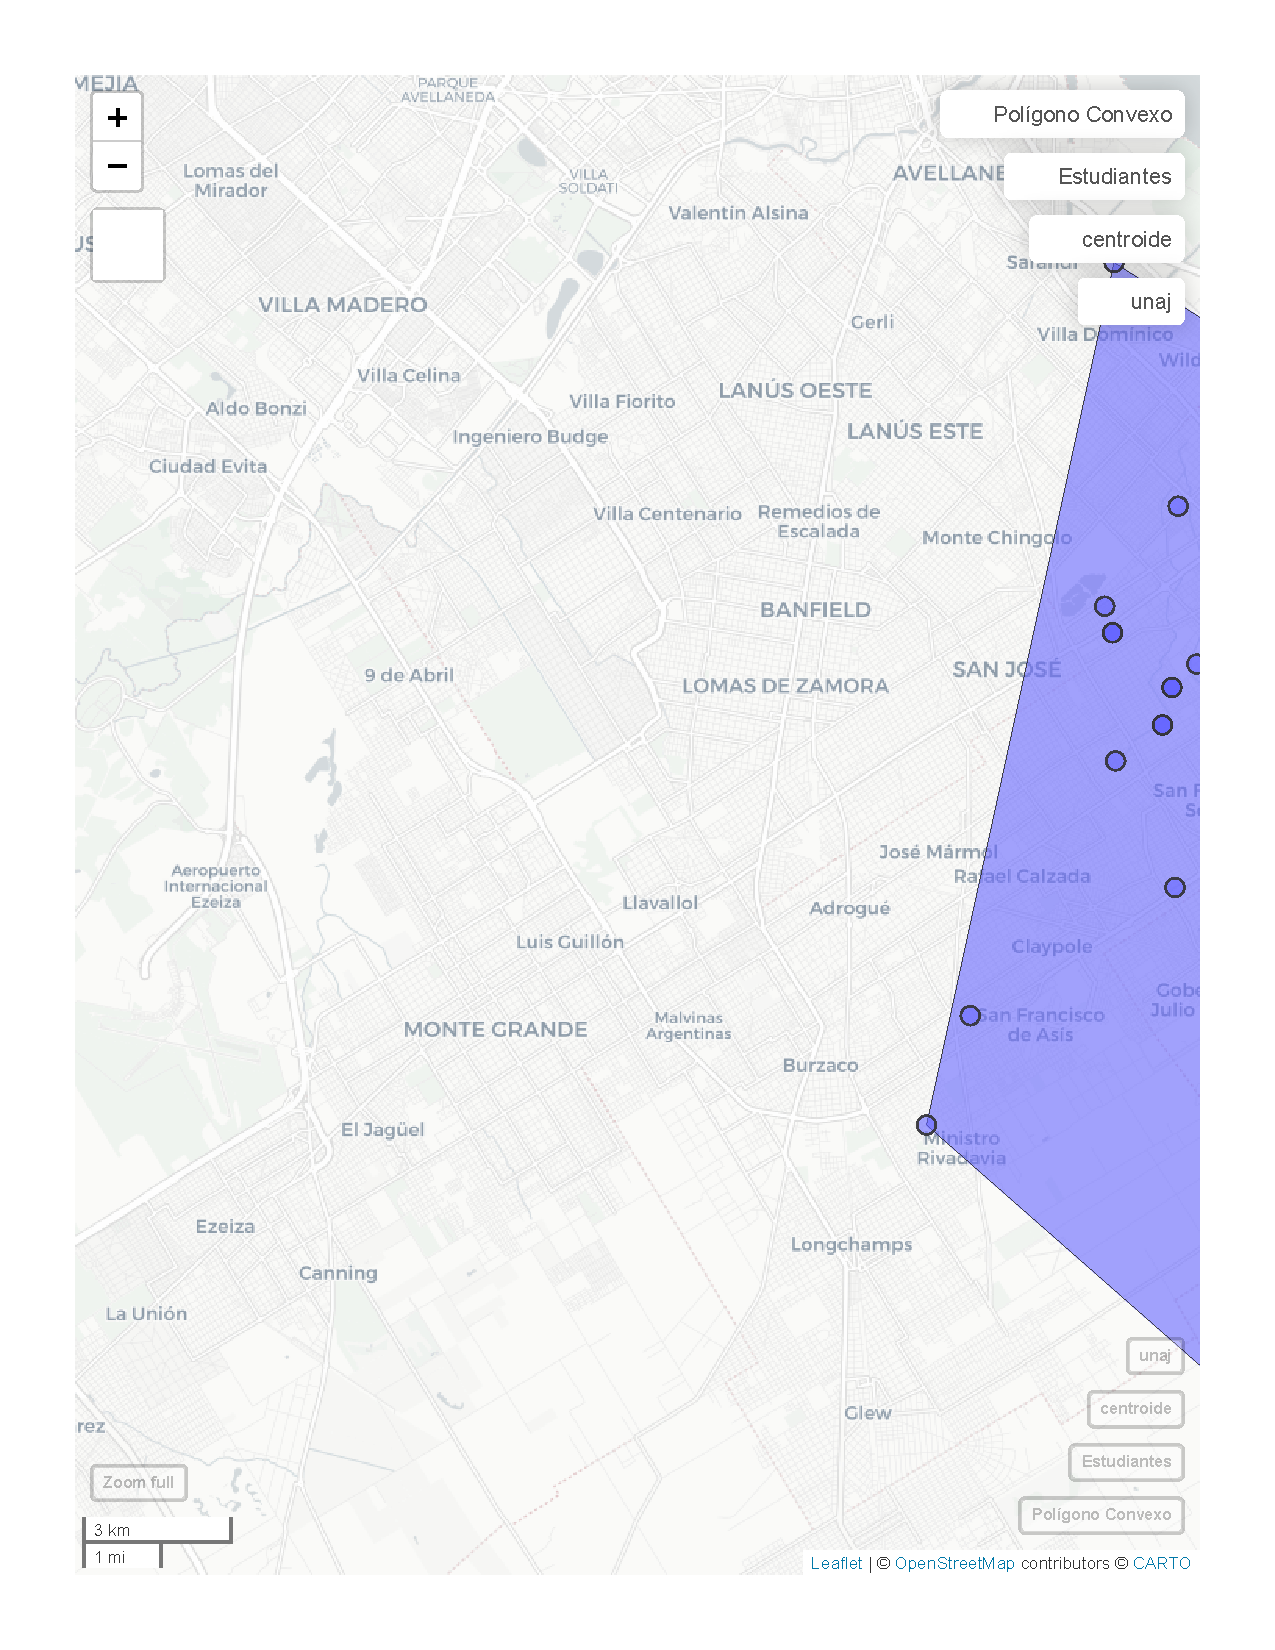
\includegraphics{./geo_files/figure-pdf/geo_mapa-1.pdf}

\hypertarget{anuxe1lisis-espaciales-1}{%
\section{Análisis espaciales}\label{anuxe1lisis-espaciales-1}}

Todos solemos tener intuiciones acerca de como el espacio influye en las
decisiones de las personas.

La georefeenciación es un proceso que consta en asignarle unas
coordenadas geográficas específicas a algún hecho, aun cuando este
cambie en tiempo y espacio, como por ejemplo, la trayectoria recorrida
en una bicicleta. Todo lo que se pueda decir que sucede en un espacio
geográfico es plausible de aplicarle una georeferenciación. La cantidad
de información georeferenciada viene creciendo a pasos agigantados en
los últimos tiempos. Esto es especialmente notoria en ciertos datos
importantes que no cambian seguido en el tiempo, como por ejemplo, las
divisiones políticas de los países. Este tipo de datos ya suelen ser de
libre disponibilidad y son un soporte genérico para cualquier
investigación específica.

El talón de Aquiles de una investigación que quiera hacer uso de los
mapas modernos es que cada investigador debe agregar los datos
específicos de su investigación que quiera georeferenciar. Expresado en
la jerga actual, se dice que cada investigador debe agregar una
\emph{capa}~específica que contenga sus datos para luego, si lo desea,
relacionarla con los otros datos genéricos que se almacenan en otras
capas genéricas. Para fijar las ideas, si yo quiero realizar una
investigación con los estudiantes de la Universidad voy a tener que
tener georeferenciada la ubicación de cada uno de ellos. Como sucede con
cualquier observación o medición, cualquier dato preciso se puede
agrupar después pero la inversa no es posible. Por ejemplo si tengo el
municipio en donde vive cada estudiantes podré hacer un mapa que coloree
los polígonos de los municipios en función de la cantidad de estudiantes
(\href{https://datavizcatalogue.com/ES/metodos/mapa_coropletico.html}{\emph{Colorpleth}})
pero no podré hacer un
\href{https://datavizcatalogue.com/ES/metodos/mapa_de_puntos.html}{mapa
de puntos}, porque este requiere las coordenadas exactas donde vive cada
estudiante. En cambio, si tengo las coordenadas puedo hacer tanto el
mapa de puntos como una graficación de los polígonos de cada municipio.

La tecnología que permite manejar y dibujar un mapa trabajando con
varias capas de información georeferenciada se llama GIS (Geographical
Information System). Históricamente De forma más contemporánea, los GIS
online, también permitieron que no sea (tan) necesario como antes la
construcción de mapas sobre un plano mediante una única proyección. La
razón es que en la actualidad, la conocida función de «zoom» de
programas como google maps (o su antecesor el google earth) ajusta de
modo automático entre diferentes proyecciones. En otras palabras, se
actualiza una proyección diferente para cada nivel de zoom.

En otras palabras, los mapas online de ahora son la unión de:

\begin{itemize}
\item
  Una mejor información satelital en cuanto a fotos satelitales y
  cálculos de distancias.
\item
  Una gran cantidad de información georeferenciada (capas), muchas
  (ahora) construidas por voluntarios desde sus teléfonos celulares
\item
  Una mejor procesamiento digital de mayor información disponible,
  mediante programas GIS y (ahora) también web, que vuelve menos
  relevante la construcción de un mapa sobre un plano.
\end{itemize}

\bookmarksetup{startatroot}

\hypertarget{anuxe1lisis-de-textos}{%
\chapter{Análisis de textos}\label{anuxe1lisis-de-textos}}

\hypertarget{insumos-de-la-encuesta-1}{%
\section{Insumos de la encuesta}\label{insumos-de-la-encuesta-1}}

El insumo de estos análisis es una serie de preguntas de respuesta
abierta. Sin embargo, dado el formato específico de la pregunta se trata
de un dato que, si bien no puede considerarse estructurado, se aleja un
poco de otros ejemplos de datos no estructurados como los textos
provenientes de entrevistas en profundidad, de canciones o de discursos
presidenciales.

\begin{figure}

{\centering 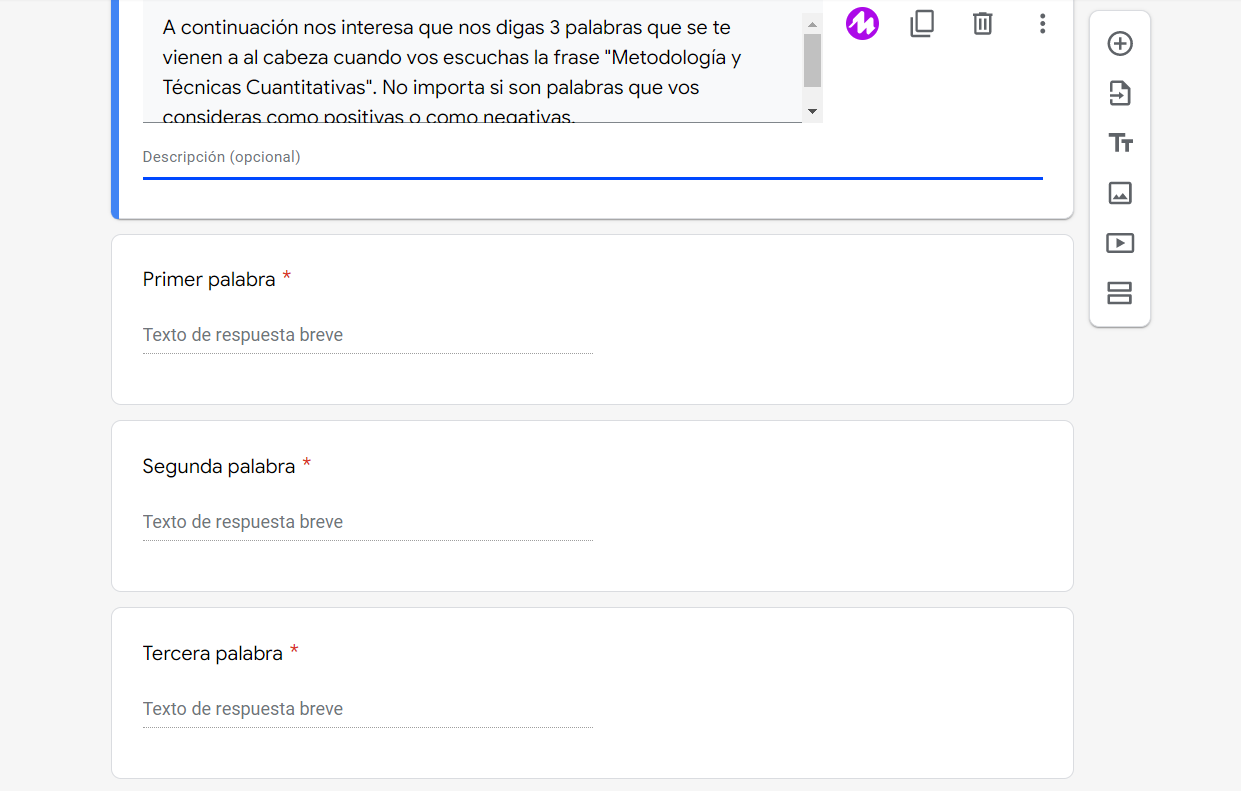
\includegraphics[width=6.25in,height=\textheight]{./Inputs/Images/preguntas_texto.png}

}

\caption{pregunta\_texto}

\end{figure}

En este caso, como puede observarse en la imagen se trata de 3 palabras
por cada encuestado. Expresado en el léxico de una matriz de datos (o
base de casos x variables), se trata de 3 columnas por cada fila.

\hypertarget{preparaciuxf3n-de-los-datos}{%
\section{Preparación de los datos}\label{preparaciuxf3n-de-los-datos}}

Para facilitar el siguiente análisis lo que primero debemos realizar es
un ``alargamiento'' de la base de datos original para pasar a tener una
sola columna y más filas que, en principio, se repetirían 3 veces.

Luego, sigue el proceso de limpieza de las palabras. Se pasa todo a
minúscula, se eliminan los puntos, los números y toda palabra vacía de
significado como los pronombres, artículos y preposiciones. Finalmente
se hace un proceso en donde se intenta llevar todas las palabras a su
raíz (\emph{stemming}) para así poder interpretar como una misma palabra
a palabras que, por ejemplo, cambian el género (gato, gata) o el número
(gato, gatos). Ahora sí, ya estamos en mejores condiciones de empezar
nuestro análisis del texto.

\hypertarget{primeras-aproximaciones}{%
\section{Primeras aproximaciones}\label{primeras-aproximaciones}}

Dado que los pasos anteriores nos permitieron estructurar bastante los
datos, ahora es más fácil realizar los típicos análisis que se realizan
a los datos estructurados. Para comenzar vamos a realizar una simple
tabla de conteo, con su respectivo porcentaje, y luego vamos a realizar
un gráfico de barras. Finalmente realizaremos una nube de palabras.

\begin{longtable}{lrr}
\caption*{
{\large Frecuencia y porcentajes de palabras}
} \\ 
\toprule
Palabra & Cantidad & Porcentaje \\ 
\midrule
investigación & 58 & $19.21\%$ \\ 
encuesta & 34 & $11.26\%$ \\ 
método & 31 & $10.26\%$ \\ 
estadística & 26 & $8.61\%$ \\ 
numeros & 22 & $7.28\%$ \\ 
datos & 14 & $4.64\%$ \\ 
cantidad & 13 & $4.30\%$ \\ 
conocimiento & 10 & $3.31\%$ \\ 
porcentaje & 9 & $2.98\%$ \\ 
técnica & 8 & $2.65\%$ \\ 
análisis & 6 & $1.99\%$ \\ 
contar & 5 & $1.66\%$ \\ 
herramientas & 5 & $1.66\%$ \\ 
camino & 4 & $1.32\%$ \\ 
científico & 4 & $1.32\%$ \\ 
difícil & 4 & $1.32\%$ \\ 
investigar & 4 & $1.32\%$ \\ 
proyecto & 4 & $1.32\%$ \\ 
conocer & 3 & $0.99\%$ \\ 
información & 3 & $0.99\%$ \\ 
medición & 3 & $0.99\%$ \\ 
modos & 3 & $0.99\%$ \\ 
objetivos & 3 & $0.99\%$ \\ 
practica & 3 & $0.99\%$ \\ 
procedimiento & 3 & $0.99\%$ \\ 
proyectos & 3 & $0.99\%$ \\ 
trabajosamente & 3 & $0.99\%$ \\ 
cifras & 2 & $0.66\%$ \\ 
cuestionarios & 2 & $0.66\%$ \\ 
estudios & 2 & $0.66\%$ \\ 
personas & 2 & $0.66\%$ \\ 
planificación & 2 & $0.66\%$ \\ 
pregunta & 2 & $0.66\%$ \\ 
promedios & 2 & $0.66\%$ \\ 
\bottomrule
\end{longtable}

Como en muchas otras situaciones, lo que se puede mostrar en forma de
tabla también se puede graficar con algún tipo de gráfico. En este caso
haremos un gráfico de barras con los datos anteriores.

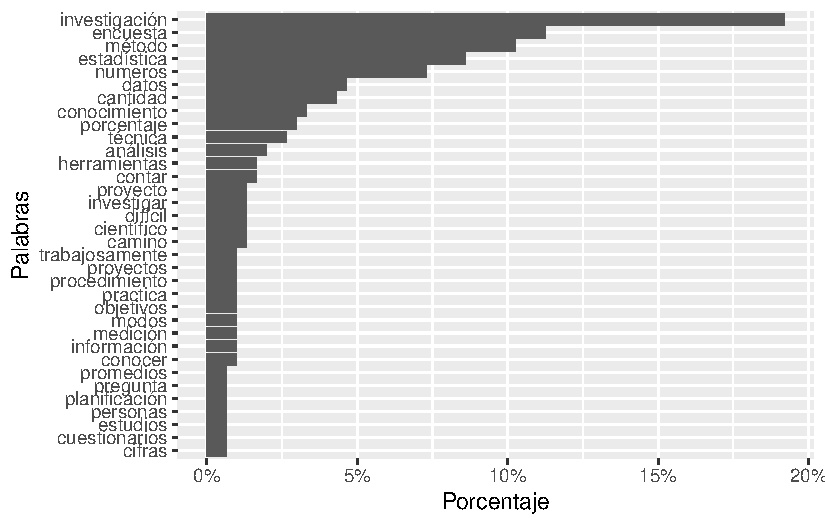
\includegraphics{./text_files/figure-pdf/grafico_conteo-1.pdf}

\hypertarget{nube-de-palabras}{%
\section{Nube de palabras}\label{nube-de-palabras}}

La nube de palabras es una técnica de visualización que funciona bien
cuando los insumos son palabras y estan presentan una gran
heterogeneidad en los valores de sus frecuencias.

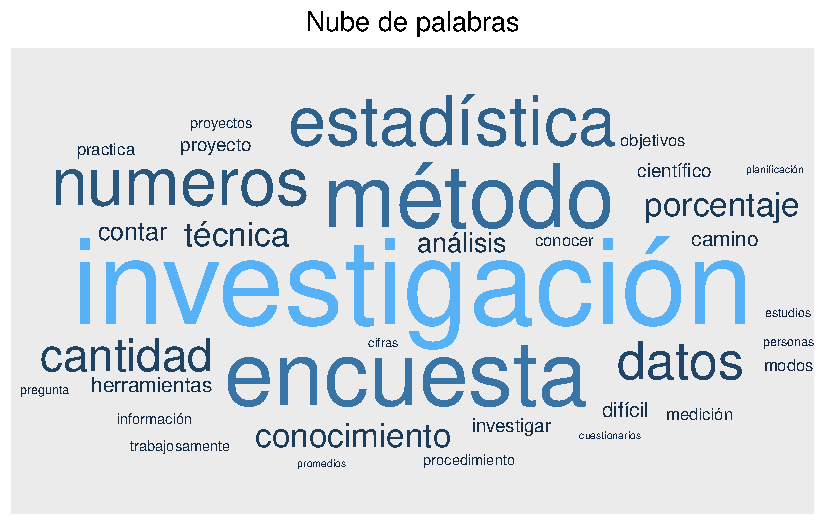
\includegraphics{./text_files/figure-pdf/text_nube_general-1.pdf}

\hypertarget{anuxe1lisis-bivariado-de-palabras}{%
\section{Análisis bivariado de
palabras}\label{anuxe1lisis-bivariado-de-palabras}}

\begin{longtable}{lrr}
\caption*{
{\large Frecuencia y porcentajes de palabras según cantidad de materias aprobadas}
} \\ 
\toprule
 & \multicolumn{2}{c}{Cantidad de materias aprobadas} \\ 
\cmidrule(lr){2-3}
Palabra & Hasta 15 & Más de 15 \\ 
\midrule
investigación & $20.00\%$ & $20.00\%$ \\ 
encuesta & $12.22\%$ & $10.48\%$ \\ 
método & $11.11\%$ & $10.48\%$ \\ 
estadística & $7.78\%$ & $11.43\%$ \\ 
numeros & $7.78\%$ & $6.67\%$ \\ 
cantidad & $4.44\%$ & $4.76\%$ \\ 
datos & $3.33\%$ & $7.62\%$ \\ 
técnica & $3.89\%$ & NA \\ 
conocimiento & $2.78\%$ & $4.76\%$ \\ 
porcentaje & $2.78\%$ & $3.81\%$ \\ 
contar & $2.22\%$ & NA \\ 
investigar & $2.22\%$ & NA \\ 
científico & NA & $3.81\%$ \\ 
análisis & $1.67\%$ & $2.86\%$ \\ 
camino & $1.67\%$ & NA \\ 
conocer & $1.67\%$ & NA \\ 
difícil & $1.67\%$ & NA \\ 
proyectos & $1.67\%$ & NA \\ 
herramientas & $1.11\%$ & $2.86\%$ \\ 
trabajosamente & NA & $2.86\%$ \\ 
información & $1.11\%$ & NA \\ 
medición & $1.11\%$ & NA \\ 
modos & $1.11\%$ & NA \\ 
personas & $1.11\%$ & NA \\ 
planificación & $1.11\%$ & NA \\ 
pregunta & $1.11\%$ & NA \\ 
procedimiento & $1.11\%$ & NA \\ 
promedios & $1.11\%$ & NA \\ 
proyecto & $1.11\%$ & $1.90\%$ \\ 
estudios & NA & $1.90\%$ \\ 
objetivos & NA & $1.90\%$ \\ 
practica & NA & $1.90\%$ \\ 
\bottomrule
\end{longtable}

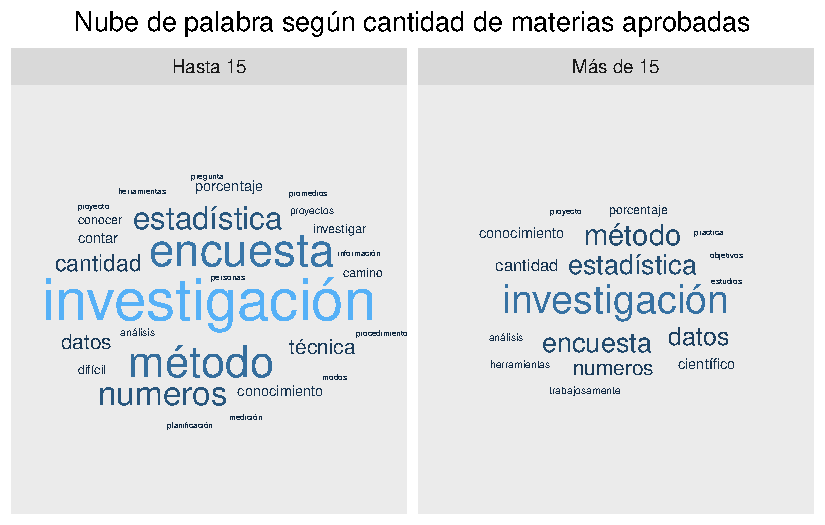
\includegraphics{./text_files/figure-pdf/nube_palabras_grupo-1.pdf}

\bookmarksetup{startatroot}

\hypertarget{anuxe1lisis-de-redes}{%
\chapter{Análisis de redes}\label{anuxe1lisis-de-redes}}

\hypertarget{insumos-de-la-encuesta-2}{%
\section{Insumos de la encuesta}\label{insumos-de-la-encuesta-2}}

El insumo de estos análisis es una serie de preguntas en donde cada
estudiante debe elegir, entre todos los estudiantes de ese cuatrimestre,
a los 5 a los que más conoce. Como tal este módulo puede considerarse
como una serie de preguntas cerradas de respuesta única con la
característica saliente de que esas preguntas poseen muchas opciones
posibles. En efecto, las opciones son tantas como estudiantes estén
cursando la materia. Desde un punto de vista metodológico lo importante
no es tanto que las opciones sean muchas o pocas sino que el rango de
estas es conocido y discreto.

Luego de una primera pregunta en donde el estudiante se auto identifica
en la lista se pasa a otras 5 preguntas en donde el estudiante va
eligiendo a otres compañeres a los cuales más conoce. Si no conoce a
nadie más elige la opción ``00-NO CONOZCO A NADIE MAS'' en las
siguientes preguntas.

\begin{figure}

{\centering 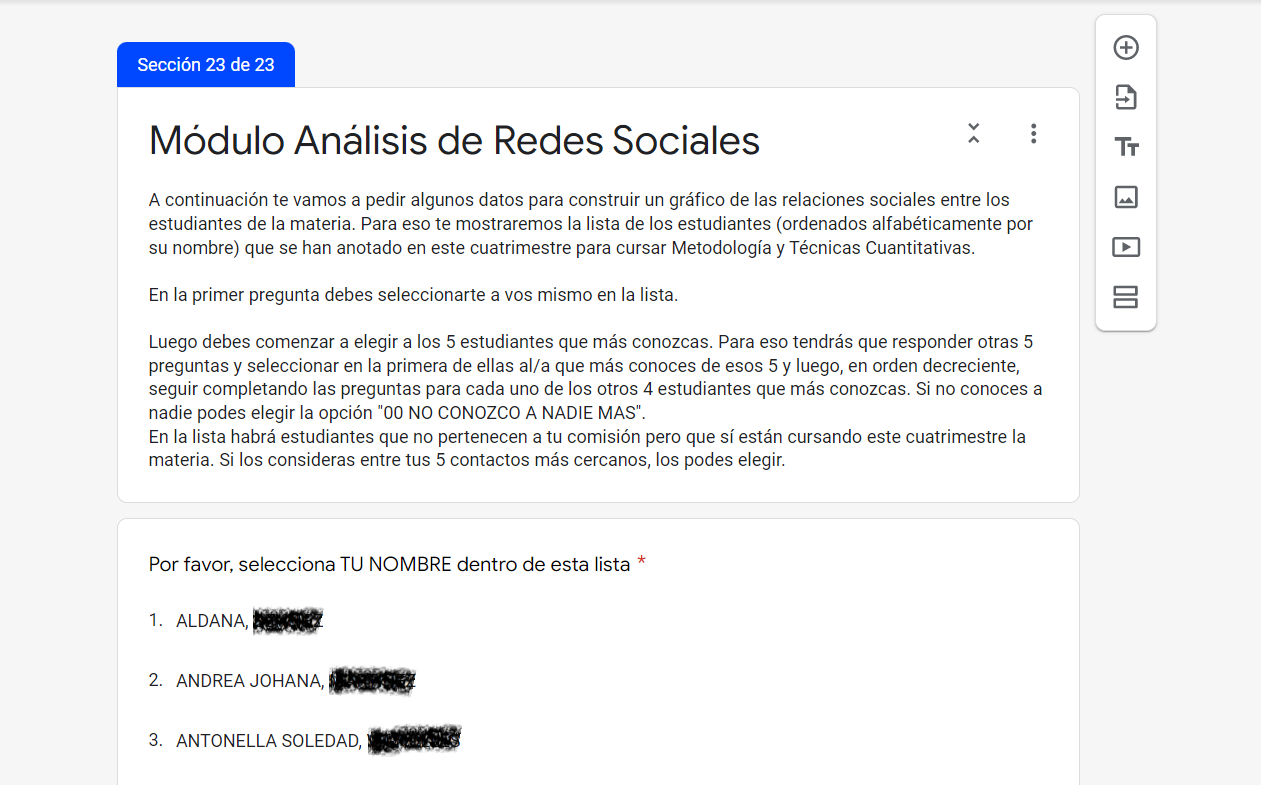
\includegraphics[width=6.25in,height=\textheight]{./Inputs/Images/pregunta_redes_1.png}

}

\caption{pregunta\_redes\_1}

\end{figure}

\begin{figure}

{\centering 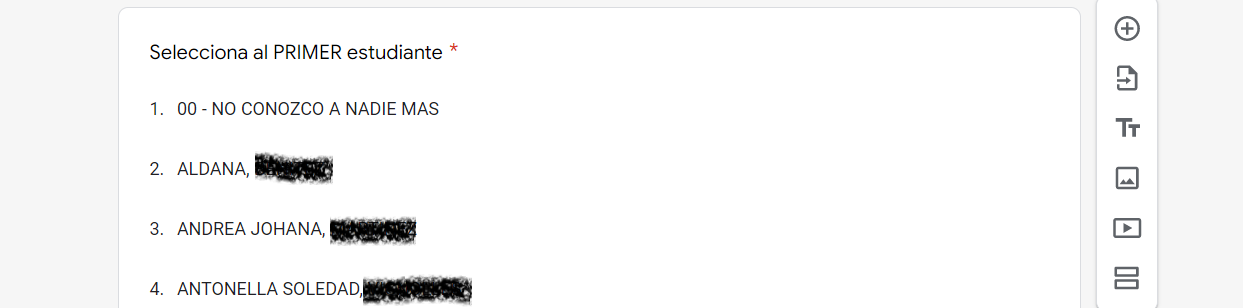
\includegraphics[width=6.25in,height=\textheight]{./Inputs/Images/pregunta_redes_2.png}

}

\caption{pregunta\_redes\_2}

\end{figure}

La explicitación de lo anterior es importante por la siguiente razón. El
análisis de redes sociales (SNA) no se suele llevar bien con la
estructura de datos conocida conocida en las ciencias sociales como
\textbf{matriz de datos} (Galtung 1973) o, más en general, como una
estructura de datos ``casos x variables''. Como lo suguiere esta última
descripción esta es una estructura afín a lo que se suele demoninar
``datos de atributos'' en donde los valores de las variables se
consideran atributos de cada uno de los casos. En cambio, en el SNA
suele ser preferible alguna de los siguientes estructura de datos que se
consideran más idóneas para representar un tipo de dato
\textbf{relacional} (Scott 2017, cap. 4):

a) Una \textbf{matriz de adyacencia} (\emph{adjacency matrix}) en donde
las filas y las columnas son asignados para los (mismos) nodos de la red
y la presencia de una relación es representada con un valor numérico. Se
dice que es una matriz cuadrada y dispersa porque tiene la misma
cantidad de filas y columnas y puede que muchas de sus celdas contengan
un valor ``0''. Se suele considerar la representación estándar de esta
técnica.

b) Una \textbf{lista de lazos} (e\emph{dge list}) en donde (sólo) se
``listan'' todas las relaciones de la red. Es una opción que, en
comparación a la opción ``a'', suele ocupar menos espacio en memoria ya
que sólo representa la presencia y/o intensidad de las relaciones entre
los nodos. En general se trata de una estructura más larga que ancha ya
que cada relación ocupa una fila y las columnas se suelen limitar
(aunque no necesariamente) a algo como ``origen'' (\emph{from}),
``destino'' (\emph{to}) e ``intensidad de la relación''.

c) Una \textbf{lista de adyacencia} (\emph{adjacency list}) que puede
considerarse un híbrido entre las opciones ``a'' y ``b''. En este caso
cada nodo se representan en una fila y cada una de ellas se ``listan''
todas sus relaciones con otros nodos. Dado lo anterior esta estructura
tiene tantas filas como nodos pero la cantidad de columnas de cada fila
es igual a la cantidad de relaciones que tenga cada nodo.

\hypertarget{breve-introducciuxf3n-al-anuxe1lisis-de-redes}{%
\section{Breve introducción al análisis de
redes}\label{breve-introducciuxf3n-al-anuxe1lisis-de-redes}}

El análisis de redes (\emph{Network Analysis} o \emph{NA}) es un enfoque
que tiene una larga historia dentro de las ciencias en general. En el
caso más particular del
\href{https://es.wikipedia.org/wiki/An\%C3\%A1lisis_de_redes\#An\%C3\%A1lisis_de_Redes_Sociales}{Análisis
de Redes Sociales} (Social \emph{Network Analysis} o \emph{SNA}) su
origen tiene 2 patas diferenciadas. Por un lado, tuvo que ver con la
invención del
\href{https://es.wikipedia.org/wiki/Sociograma}{sociograma}, el cual, a
su turno, tuvo que ver con el origen de la
\href{https://es.wikipedia.org/wiki/Sociometr\%C3\%ADa}{sociometría}. El
sociograma es una herramienta de visualización de las relaciones
sociales que conforman un grupo. Para su construcción se requiere de
datos de todos los miembros de ese grupo por lo que su utilización
muchas veces se restringue a grupos o organizaciones pequeños. En parte
por lo anterior, no son muchas las investigaciones empíricas que lo
utilizan dada la dificultad metodológica de obtener esos datos.

\begin{tcolorbox}[enhanced jigsaw, colback=white, title=\textcolor{quarto-callout-note-color}{\faInfo}\hspace{0.5em}{Sabías qué? Análisis de redes y matemática}, breakable, colbacktitle=quarto-callout-note-color!10!white, opacityback=0, opacitybacktitle=0.6, titlerule=0mm, toprule=.15mm, toptitle=1mm, leftrule=.75mm, rightrule=.15mm, bottomrule=.15mm, arc=.35mm, coltitle=black, bottomtitle=1mm, left=2mm, colframe=quarto-callout-note-color-frame]

El análisis de redes en general y el análisis de redes sociales en
particular puede considerarse como una aplicación de una teoría
matemática abstracta como es la
\href{https://es.wikipedia.org/wiki/Teor\%C3\%ADa_de_grafos}{teoría de
grafos} (\emph{Graph Theory}). Esta última se origina en un
\href{https://drive.google.com/file/d/1Vr1BQT-7GAK9ia5YbMfYul4Lwzhv3LVP/view}{clásico
artículo} de Leonard Euler de 1741 en donde trata el conocido problema
de
\href{https://es.wikipedia.org/wiki/Problema_de_los_puentes_de_K\%C3\%B6nigsberg}{los
siete puentes de Königsberg} (Euler 1741). El problema consiste en
encontrar un recorrido para cruzar a pie toda la ciudad pasando sólo una
vez por cada uno de los puentes y regresando al mismo punto de inicio.

\begin{figure}[H]

{\centering 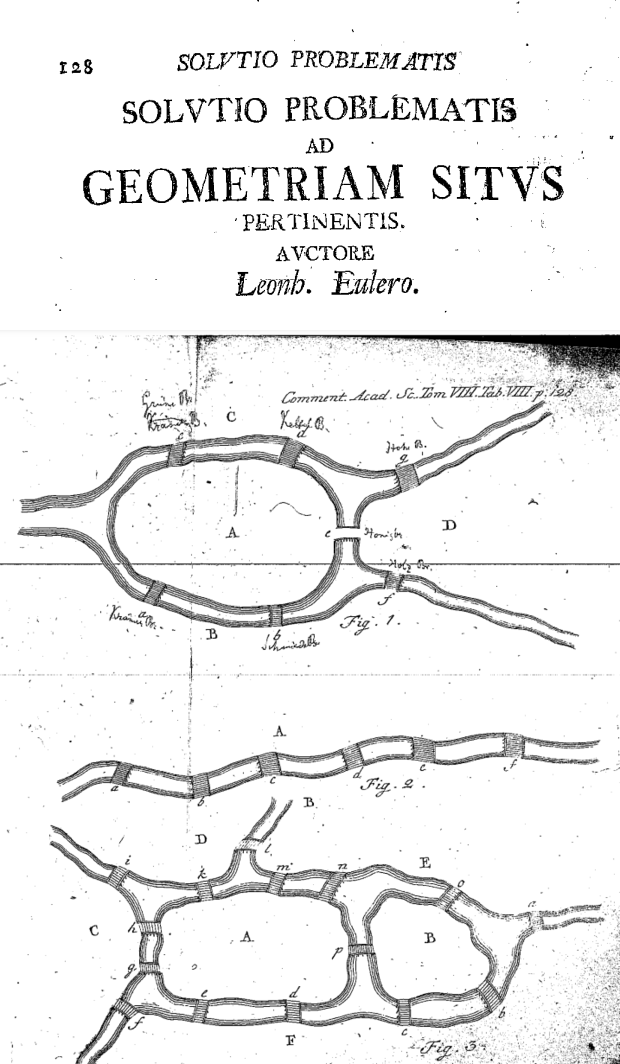
\includegraphics{./_book/Inputs/Images/euler_article.png}

}

\end{figure}

\end{tcolorbox}

Recién luego de varias décadas la visualización del sociograma se
relacionó explícitamente con la teoría de grafos, dando origen al SNA.
Si los sociogramas tenían la dificultad metodológica de su construcción,
con la incorporación de la teoría de grafos se sumó la dificultad
metodológica del análisis de esos datos. Estas 2 condiciones todavía
afectan mucho el grado de difusión de este enfoque, aunque en la
actualidad tanto la huella digital contenida en la redes sociales
virtuales (facebook, twitter, etc.) como la emergencia de programas
informáticos que facilitan el análisis ha favorecido una mayor difusión.
En parte por lo anterior, en lo que sigue se mostrará como se pueden
hacer análisis y visualizaciones de redes con datos provenientes de una
base original de casos x columnas.

\hypertarget{anuxe1lisis-y-visualizaciones}{%
\section{Análisis y
visualizaciones}\label{anuxe1lisis-y-visualizaciones}}

\hypertarget{centralidades-de-los-estudiantes-y-sus-relaciones}{%
\subsection{Centralidades de los estudiantes y sus
relaciones}\label{centralidades-de-los-estudiantes-y-sus-relaciones}}

En un grafo, los nodos (\emph{nodes}) representan a los entes
relacionados (aquí estudiantes) y las líneas o aristas (\emph{edges})
representan a las relaciones entre ellos. En este sentido, el SNA
contiene una serie de conceptos cuantitativos que tienen como insumo la
cantidad y calidad de las relaciones. Algunos de esos conceptos con
aplicables para cada nodo (p.e. estudiantes), otros son aplicables para
el conjunto de ellos (p.e. comisiones).

En el siguiente gráfico (o grafo más precisamente) se puede observar los
estudiantes del último cuatrimestre (2022 - Segundo Cuatrimestre) y las
relaciones sobre quien conoce a quien al principio de la cursada.

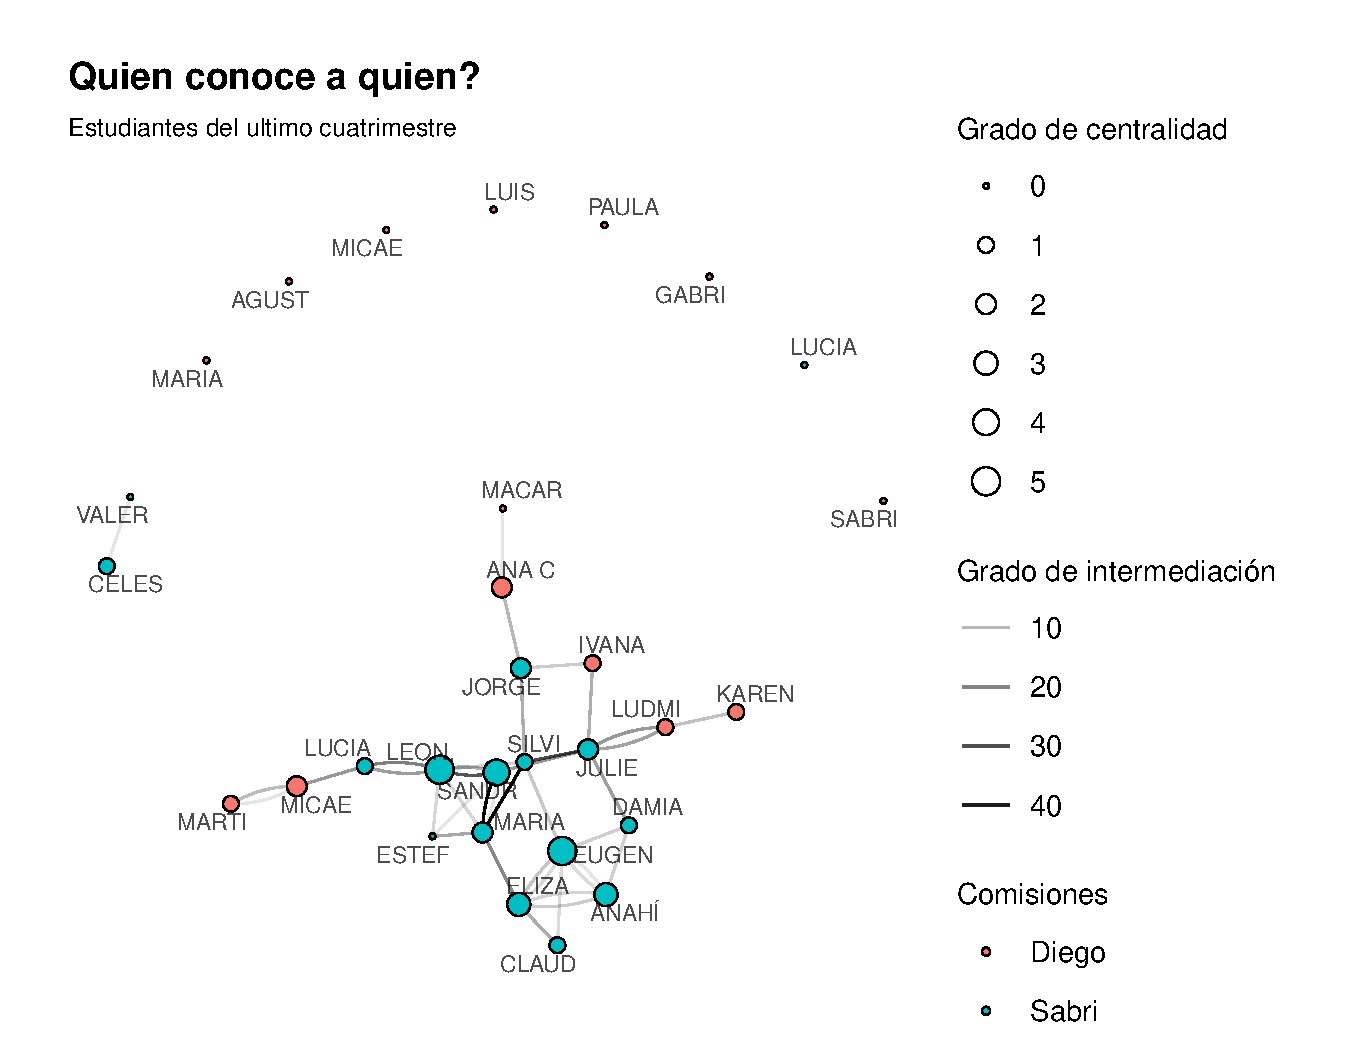
\includegraphics{./redes_files/figure-pdf/graph_last-1.pdf}

En este caso, las relaciones se visualizan con líneas. Estas pueden ser
tanto relaciones entrantes (``me conocen a mí'') o salientes (``yo
conozco a''). Para facilitar la visualización el tamaño de cada
estudiante es proporcional a la cantidad de relaciones entrantes que
podría considerarse como un indicador grueso de popularidad. En el
contexto del SNA este concepto se denomina grado de centralidad
(\emph{centrality degree}).

Otro concepto importante del SNA es el de la intermediación
(\emph{betweeness centrality}). Este puede calcularse tanto para nodos
como para las relaciones. En efecto, en el gráfico anterior se visualizó
el valor de este concepto para las relaciones (``grado de
intermediación''). El criterio que determina el valor es el número de
caminos más cortos que pasan a través de ese nodo o relación. La idea de
camino más corto es un concepto fuerte del SNA y hace referencia a cual
es el ``camino'' más corto entre un nodo (o relación) y otro nodo (u
otra relación) teniendo en cuenta las relaciones existentes. Por
ejemplo, hay personas que no son necesariamente populares pero ocupan
una posición ventajosa en la red social porque ellos tienen una
información que les puede servir a otros. Pensemos en la típica
situación en donde necesitamos pedirle un favor a alguien popular pero
la unica manera de acceder a él es a través de su secretaria/o. Este
última/o puede no ser popular pero tiene un nivel alto de
intermediación.

Por último, aplicaremos un concepto del SNA que, intuitivamente, remite
a la idea de influencia. Aquí el criterio de esta centralidad es que
aquellos nodos que están conectados con otros nodos que, a su turno,
están conectados con otros \ldots{} tienen más influencia que aquellos
que están conectados con otros nodos pero que, a su turno, estos no
están conectados con nadie. En este sentido, no es lo mismo conocer a 5
personas que son pocos conocidos que conocer a 5 personas que son muy
conocidas por otros. Esta es la diferencia principal entre alguien
``popular'' y un ``influencer''. Ejemplo de conceptos del SNA que se
acercan a esta intuición pueden considerarse la centralidad del vector
propio (\emph{eigenvector centrality),} la centralidad que se usa en el
rankeo de las páginas de google (google page rank) y la centralidad de
Katz (\emph{katz centralit}y). Aquí sólo calcularemos la centralidad del
propio vector.

\begin{longtable}{lrrr}
\toprule
Estudiante & G. centralidad & G. intermediación & G. de influencia \\ 
\midrule
LEON, & 5 & $33.00$ & $0.00$ \\ 
EUGEN & 5 & $7.33$ & $1.00$ \\ 
SANDR & 4 & $40.33$ & $0.00$ \\ 
ELIZA & 3 & $18.50$ & $0.87$ \\ 
ANAHÍ & 3 & $2.33$ & $0.87$ \\ 
MICAE & 2 & $8.00$ & $0.00$ \\ 
ANA C & 2 & $0.00$ & $0.00$ \\ 
MARIA & 2 & $51.33$ & $0.00$ \\ 
JORGE & 2 & $9.00$ & $0.00$ \\ 
JULIE & 2 & $40.00$ & $0.00$ \\ 
\bottomrule
\end{longtable}

Como puede observarse en la tabla anterior (sólo se muestran los 10
casos con mayor grado de centralidad), los valores de los diferentes
conceptos algunas veces son similares y otras veces no. Esto es
razonable ya que cada concepto utiliza un criterio diferente de
centralidad. Dada la pluralidad de conceptos de centralidad que existen
en el SNA siempre es conveniente explicitar con cual se está trabajando.

\bookmarksetup{startatroot}

\hypertarget{referencias-bibliogruxe1ficas}{%
\chapter*{Referencias
bibliográficas}\label{referencias-bibliogruxe1ficas}}
\addcontentsline{toc}{chapter}{Referencias bibliográficas}

\markboth{Referencias bibliográficas}{Referencias bibliográficas}

\hypertarget{refs}{}
\begin{CSLReferences}{1}{0}
\leavevmode\vadjust pre{\hypertarget{ref-euler1741}{}}%
Euler, Leonard. 1741. {«Solutio problematis ad geometriam situs
pertinentis»}. \emph{Commentarii academiae scientiarum Petropolitanae}
8: 128-40.

\leavevmode\vadjust pre{\hypertarget{ref-galtung1973}{}}%
Galtung, Johan. 1973. \emph{Teoría y Método de la Investigación Social}.
Vol. I. Buenos Aires: Eudeba.

\leavevmode\vadjust pre{\hypertarget{ref-scott2017}{}}%
Scott, John. 2017. \emph{Social Network Analysis}. 4th ed. London: Sage
Publications.

\end{CSLReferences}



\end{document}
